\documentclass[11pt]{article}
\usepackage[a4paper,margin=21mm]{geometry}
\usepackage[no-math]{fontspec}
\setmainfont{Latin Modern Roman}
\newfontfamily\CJKfont{Noto Serif CJK SC}
\XeTeXlinebreaklocale "zh"
\XeTeXlinebreakskip=0pt plus 1pt
\usepackage{amsmath,amssymb,amsthm,amscd,graphicx,color}
\usepackage{xurl}
\usepackage[unicode,hidelinks]{hyperref}
\allowdisplaybreaks
\setlength\emergencystretch{3em}
\numberwithin{equation}{section}

\numberwithin{equation}{section}

\newtheorem{Theorem}{Theorem}[section]
\newtheorem*{Theorem*}{Theorem}
\newtheorem{Corollary}[Theorem]{Corollary}
\newtheorem{Lemma}[Theorem]{Lemma}
\newtheorem{Proposition}[Theorem]{Proposition}
\newtheorem{Conjecture}[Theorem]{Conjecture}
 { \theoremstyle{definition}
\newtheorem{Definition}[Theorem]{Definition}
\newtheorem{Note}[Theorem]{Note}
\newtheorem{Example}[Theorem]{Example}
\newtheorem{Remark}[Theorem]{Remark} }

\graphicspath{{./images/} }

\makeatletter\newlabel{section_recovering_q_series}{{4}{}{Original source locator}{}{}}\makeatother
\makeatletter\newlabel{section_connected_sum}{{5}{}{Original source locator}{}{}}\makeatother
\begin{document}
\begin{center}\Large Spin-c refined two-variable series invariance for reduced plumbing trees with invertible linking matrix\end{center}
\noindent\textbf{Stable ID:} 1090\quad\textbf{Author:} Song Jin Ri\par
\noindent\textbf{Work:} Refined and Generalized $\hat{Z}$ Invariants for Plumbed 3-Manifolds\par
\noindent\textbf{Source:} \url{https://sigma-journal.com/2023/011/}\par
\noindent\textbf{Version:} Official SIGMA 19 (2023) article 011, DOI 10.3842/SIGMA.2023.011; journal PDF and native TeX acquired 2026-09-30, exact bytes pinned by SHA256\par
\noindent\textbf{Rights:} CC BY 4.0. Authors retain copyright. \url{https://creativecommons.org/licenses/by/4.0/}. Reuse and typesetting adaptation; original language and mathematical content preserved.\par
\noindent\textbf{Difficulty (prior selection preserved):} {\CJKfont H2: The proof combines reduction of Neumann-move sequences with an explicit chamber-dependent regularization of lattice theta sums. It tracks changes of linking signatures, Spin-c representatives, pseudo-branch signs and chamber choices through all three move types. The blow-up and bridge-collapse cases require different binomial coefficient convolution identities to match the refined powers of t as well as the quadratic q exponents.}\par
\medskip\noindent\textbf{Editorial boundary note (not author text):} Complete original Theorem3.5, full reduction of Neumann-move sequences in Proposition3.4, and every sign/chamber/pseudo-branch case of the refined invariance proof. All linking/Spin-c and formal constant-term/theta conventions, binomial coefficients, reduced/pseudo plumbing definitions, chamber constraints and regulated discriminant definitions are retained. The author gives the local matrix and binomial formulas, and transparently describes the repeated positive-sign/pseudo-bridge and multiple-pseudo-vertex cases as similar extensions; these exact statements and their inputs are preserved without editor derivations. Original graph assets and a separately marked editable transcription of every printed weight/move label are included. One principal reduced-plumbing invariant outcome expressly announced in the introduction; supporting reduction and convolution pieces are not extra counts. Subsequent recovering limits, examples, conjectures and connected-sum outcome are excluded. Printed source signs and formula irregularities are retained without mathematical correction.\par
\noindent\textbf{External original reference section\_recovering\_q\_series:} Original subsequent recovery/limit section, source479–871. The retained tree convention mentions its scope; this separate limit outcome is not an input to the selected reduced-plumbing invariance proof.\par
\noindent\textbf{External original reference section\_connected\_sum:} Original later connected-sum section, source872–985. Mentioned only in the tree/disconnected convention; not used in the selected theorem.\par
\medskip\hrule\medskip\noindent\textbf{Author text begins below.}\par
\setcounter{section}{1}
% Original source lines 68--436
\section[Plumbed 3-manifolds and q-series]{Plumbed 3-manifolds and $\boldsymbol{q}$-series}
\label{section_plumbed_3-manifolds}

In this section we review some known facts about plumbed 3-manifolds and their invariants, and we set up notational conventions.

\subsection{Plumbing graphs}\label{subsection_plumbing_graphs}

A \textit{plumbing graph} is a finite weighted graph $ \Gamma $, that is, a graph consisting of a finite number of vertices and edges together with the data of integer weights associated to vertices. In Section~\ref{section_plumbed_3-manifolds}--\ref{section_recovering_q_series}, we will assume that $ \Gamma $ is a tree, and we will consider disconnected plumbings in Section~\ref{section_connected_sum}.

Let $ V $ be the set of vertices of $ \Gamma $. For each vertex $ v\in V $, $ m_v $~denotes the weight of the vertex~$ v $, and the degree $ \deg(v) $ describes the number of edges connected to the vertex. Let $ s=|V| $ be the cardinality of the set $ V $. Then we define the symmetric $ s\times s $ matrix $ M=M(\Gamma) $, called \textit{linking matrix} of $ \Gamma $, by
\begin{equation*}
	M_{v_1,v_2}=
	\begin{cases}
		m_v,&\text{if } v_1=v_2=v,\\
		1,&\text{if }v_1, \ v_2 \text{ are connected by an edge},\\
		0,&\text{otherwise}.
	\end{cases}
	\qquad v_i\in V.
\end{equation*}

From $ \Gamma $, we can construct plumbed 3-manifolds in the following way: we first obtain the framed link $ L(\Gamma) $ in $S^3=\partial B^4$ by taking an unknot with framing $ m_v $ for each vertex $ v $ and making these unknots forming Hopf links whenever corresponding vertices are connected by an edge, e.g., see Figure \ref{fig_framed_link}.
\begin{figure}[t]
	\centering
	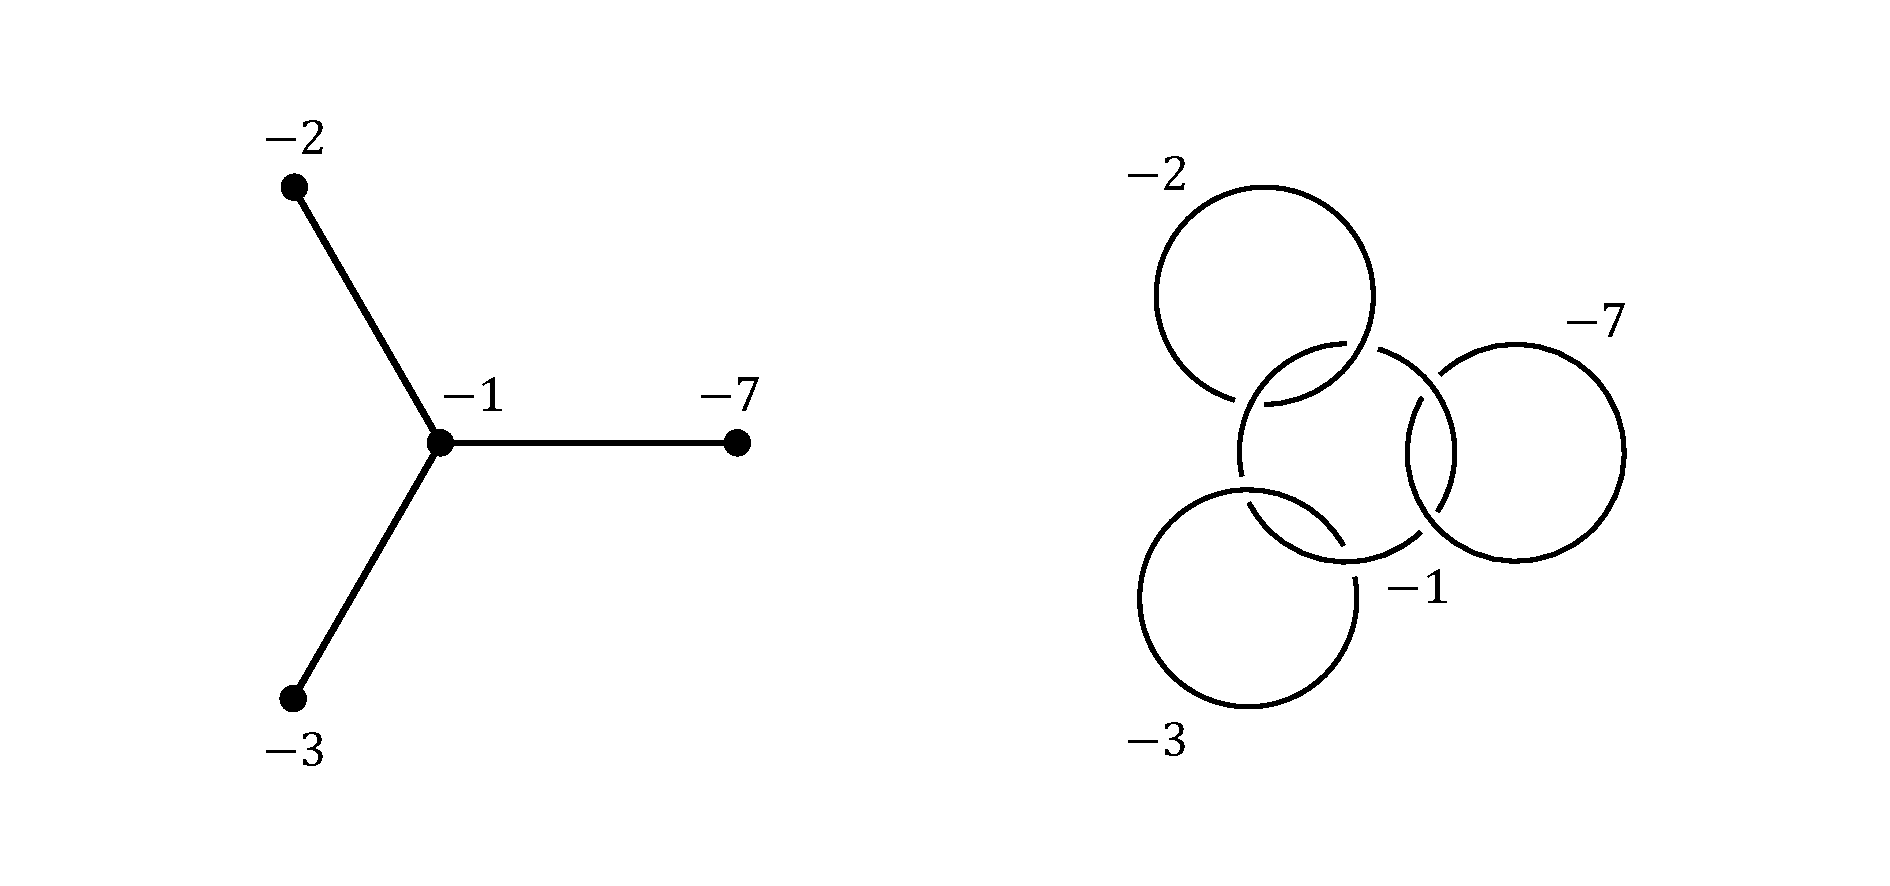
\includegraphics[scale=0.39]{../assets/1090/./images/framed_link.pdf}
	\caption{A plumbing graph $ \Gamma $ on the left and its associated framed link $ L(\Gamma) $ on the right.}
	\label{fig_framed_link}
\end{figure}
By attaching two-handles to $ B^4 $ along $ L(\Gamma) $, we get the 4-manifold, denoted by $ W(\Gamma) $. It can be also obtained by plumbing disk bundles over $ S^2 $ with Euler numbers~$ m_v $. Then its boundary $ Y=Y(\Gamma)=\partial W(\Gamma) $ is the closed and oriented 3-manifold obtained by Dehn surgery from $ L(\Gamma) $ whose first homology is
\[
H_1(Y)\cong \mathbb{Z}^s/M\mathbb{Z}^s.
\]

Two different plumbing graphs can represent the same homeomorphism class of $ Y(\Gamma) $. This happens if and only if they are related by a finite sequence of Neumann moves~\cite{neumann} depicted in Figure \ref{fig_neumann_moves}.
\begin{figure}[t]
	\centering
	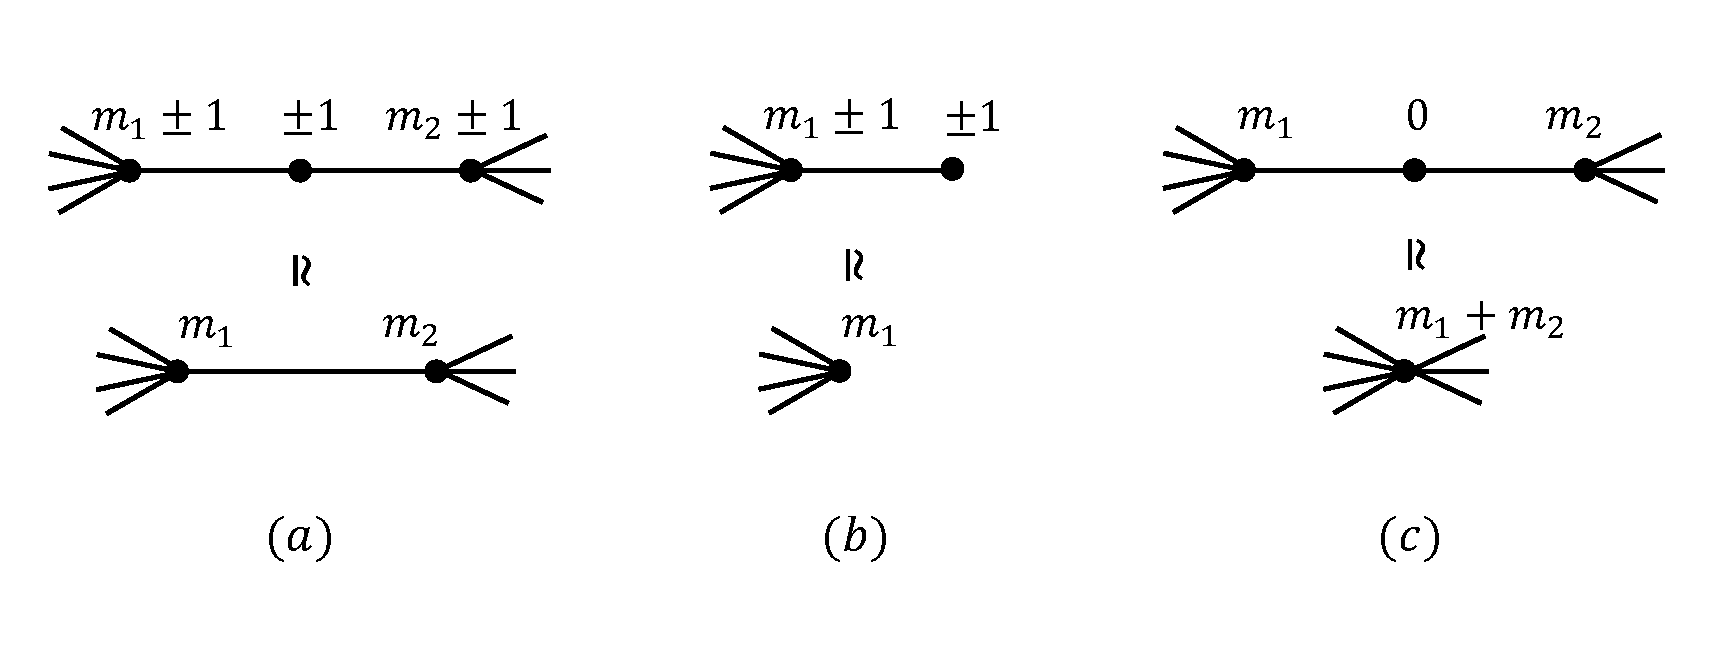
\includegraphics[scale=0.4]{../assets/1090/images/neumann_moves.pdf}
	\caption{Neumann moves on plumbing graphs that realize homeomorphic 3-manifolds.}
	\label{fig_neumann_moves}
\end{figure}

For the purposes of this paper, we establish some terminology of plumbings that can be helpful for understanding the structures of plumbing graphs. Given a graph $ \Gamma $, we divide the set $ V $ of vertices into three disjoint subsets $ V_1$, $V_2 $ and $ V_h $ with respect to the degree of vertices as following:
\begin{gather*}
	V_1=\{v\in V\mid \deg(v)=1\}, \qquad V_2=\{v\in V\mid \deg(v)=2\}, \\
	V_h=\{v\in V\mid \deg(v)=2+p_v\geq 3, \, p_v\in \mathbb{Z}_{>0} \}.
\end{gather*}
Then we name the elements of $ V_1$, $V_2 $ and $ V_h $ by \textit{valency one}, \textit{valency two} and \textit{high-valency vertices}, respectively.

Assume that $ \Gamma $ has at least one high-valency vertex. Choose a high-valency vertex $ w\in V_h $ among them. Then $ w $ has \textit{arm}s as many as its degree $ \deg(w) $, where an arm means a part of graph, starting from a given high-valency vertex, possibly going through only a finite number of valency two vertices and ending at a valency one or another high-valency vertex. If an arm starts from $ w $ and ends at a valency one vertex $ v\in V_1 $, then we call it a \textit{branch} from $ w $ to $ v $ and denote it by $ \Gamma_{wv} $. An arm starting from a high-valency vertex $ w_1\in V_h $ and ending at another high-valency $ w_2\in V_h $ is called a \textit{bridge} between $ w_1 $ and $ w_2 $, denoted by $ \Gamma_{w_1,w_2} $. For example, two graphs in Figure~\ref{fig_neumann_moves}\,(a) have bridges between $ m_1 $ and $ m_2 $ for the bottom one or from $ m_1\pm 1 $ to $ m_2\pm 1 $ for the top, respectively, and the top graph in Figure \ref{fig_neumann_moves}\,(b) has a branch from $ m_1\pm 1 $ to $ \pm 1 $.

Since a branch $ \Gamma_{wv} $ from $ w $ to $ v $ can be thought as a linear plumbing, the following continued fraction
\begin{equation}\label{eqn_continued_fraction}
	m_w'=m_w-\cfrac{1}{u_1-\cfrac{1}{u_2-\cfrac{1}{\ddots - \cfrac{1}{m_v}}}}
\end{equation}
can give us the information of the branch. It is actually a complete invariant under the Neumann moves creating or annihilating valency two vertices along the branch. In \eqref{eqn_continued_fraction}, $ m_w $ is the weight of the starting high-valency vertex of the branch $ \Gamma_{wv} $, $ u_i $s represent the weights of valency two vertices on the linear plumbing between $ w $ and $ v $, and $ m_v $ is the weight of the ending valency one vertex. If the continued fraction $ m_w' $ of $ \Gamma_{wv} $ is an integer, the branch is called \textit{pseudo} branch because it can be annihilated or removed by a sequence of Neumann moves. For example, the top graph in Figure \ref{fig_neumann_moves}\,(b) has a pseudo-branch $\Gamma_{m_1\pm1, \pm1}$.\footnote{By abuse of notation, we often use the weights to denote the vertices where the meaning is clear in the context.} A high-valency vertex is $w\in V_h$ called a \textit{pseudo} high-valency vertex if it satisfies the following condition
\[
\deg(w) - n_w = 1, 2,
\]
where $n_w$ denotes a number of pseudo branches connected to the vertex $w$. This means that a~pseudo high-valency vertex can be turned into a valency one or two vertex once we annihilate or collapse all of its pseudo branches by using Neumann moves.

For a given bridge $ \Gamma_{w_1,w_2} $ between two high-valency vertices $ w_1,w_2\in V_h $, we also examine the continued fraction of valency two vertices laid on the bridge if they exist. The bridge is called a \textit{pseudo} bridge if it contains at least one valency two vertex and the continued fraction is zero. A pseudo bridge can also be annihilated by a sequence of Neumann moves of type (a) and (c).

We define a plumbing graph to be \textit{reduced} if there is at least one vertex with degree greater than two and there does not exist a pseudo high-valency vertex. One can change any plumbing tree into a reduced plumbing by removing pseudo high-valency vertices by using Neumann moves. Note that removing pseudo high-valency vertex could create another pseudo high-valency vertex, hence it is needed to keep removing all pseudo high-valency vertices as they appear until there is no pseudo high-valency vertex anymore. We also notice that a plumbing without any high-valency vertex represents a lens space.

\subsection[Identification of Spin\^{}c structures]{Identification of $\boldsymbol{\text{Spin}^c}$ structures}

Let us review briefly the identification of $ \text{Spin}^c $ structures on plumbed 3-manifolds in terms of plumbing data. The affine space $ \text{Spin}^c(Y) $ in the case of $ Y=Y(\Gamma) $ for a plumbing tree $ \Gamma $ has already been studied in the Heegard--Floer homology literature \cite{heegard-floer}, and a slightly different description has been used in order to construct an invariant $ \hat{Z}_a(q) $ of the plumbed 3-manifold equipped with the $\text{Spin}^c$ structure $ a $ in~\cite{gukov}. Here we recall $ \text{Spin}^c $ structures on plumbed 3-mani\-folds $ Y(\Gamma) $ by following \cite{gukov}.

The $ \text{Spin}^c $ structures on $ Y $ can be inherited by those on the 4-manifold $ W=W(\Gamma) $ with boundary $ Y $. More explicitly, a natural identification for $ \text{Spin}^c $ structures on $ W $
\begin{equation*}
	\text{Spin}^c(W)\cong 2\mathbb{Z}^s+\vec{m}
\end{equation*}
translates into a natural identification for the plumbed 3-manifold $ Y $
\begin{equation*}
	\text{Spin}^c(Y)\cong \big(2\mathbb{Z}^s+\vec{m}\big)/\big(2M\mathbb{Z}^s\big),
\end{equation*}
where $ \vec{m} $ is the vector made of the weights $ m_v $ for $ v\in V $. Note that both identifications take the conjugation of $ \text{Spin}^c $ structures to the involution $ a\leftrightarrow -a $ on the right-hand side.

Another natural identification
\begin{equation}\label{eqn_spinc_identification_Y}
	\text{Spin}^c(Y)\cong \big(2\mathbb{Z}^s+\vec{\delta}\,\big)/\big(2M\mathbb{Z}^s\big) \cong 2\operatorname{Coker}M+\vec{\delta},
\end{equation}
can be obtained by using the map
\[
\begin{split}
	\phi\colon \ \big(2\mathbb{Z}^s+\vec{m}\big)/\big(2M\mathbb{Z}^s\big) & \xrightarrow{\cong} \big(\big(2\mathbb{Z}^s+\vec{\delta}\,\big)/\big(2M\mathbb{Z}^s\big)\big),\\
	\big[\vec{\ell}\,\,\big] & \rightarrow \big[\vec{\ell}-M\vec{u}\big],
\end{split}
\]
where $ \vec{\delta} $ is the vector of the degrees of the vertices in $ \Gamma $, and $ \vec{u}=(1,1,\dots,1) $.

\subsection[The q-series]{The $\boldsymbol{q}$-series}

The $ q $-series has been firstly proposed in \cite{gppv} aimed to categorify the WRT invariant. It was originally defined for plumbed 3-manifolds coming from negative definite plumbing graphs. For a later convenience, we recall the formula of the $ q $-series $ \hat{Z}_a(q) $ for weakly negative definite plumbed 3-manifolds following \cite{gukov} and \cite{gppv}.

Let $ \Gamma $ be a plumbing graph satisfying the weakly negative definite condition, that is, the linking matrix $ M=M(\Gamma) $ is invertible and $ M^{-1} $ is negative definite on the subspace of $\mathbb{Z}^s$ spanned by the high-valency vertices. Using identifications~\eqref{eqn_spinc_identification_Y}, fix a representative $ \vec{a}\in 2\mathbb{Z}^s+\vec{\delta} $ of a class
\[
a\in \big(2\mathbb{Z}^s+\vec{\delta}\,\big)/\big(2M\mathbb{Z}^s\big).
\]
Then the $ q $-series $ \hat{Z}_a(q) $ is defined by
\begin{equation}\label{eqn_defn_q_series}
	\hat{Z}_a(q)=(-1)^{\pi}  q^{\frac{3\sigma-\sum_v m_v}{4}} \cdot \text{CT}_{\vec{z}}\left\{ \mathcal{D}(\vec{z}) \cdot \Theta_a^{M}(\vec{z})\right\},
\end{equation}
where
\begin{equation}\label{eqn_defn_discriminant_q_series}
	\mathcal{D}(\vec{z})=\prod_{v\in V} \left(z_v-\frac{1}{z_v}\right)^{2-\deg(v)}
\end{equation}
and
\begin{equation}\label{eqn_defn_Theta_function_q_series}
	\Theta_a^{M}(\vec{z})=\sum_{\vec{\ell}\in 2M\mathbb{Z}^s+\vec{a}} q^{-\frac{(\vec{\ell},M^{-1}\vec{\ell})}{4}} \prod_{v\in V} z_v^{\ell_v}.
\end{equation}
In \eqref{eqn_defn_q_series}, $ \text{CT}_{\vec{z}}$ is the operation of taking the constant terms of the formal power series in $z_v$. Also, for the factors in front of the operation $ \text{CT}_{\vec{z}}$, $ \pi=\pi(M) $ denotes the number of positive eigenvalues of the linking matrix $ M $ and $ \sigma=\sigma(M) $ is the signature of $ M $, i.e., $ \sigma=2\pi-s $.

Note that all rational functions in \eqref{eqn_defn_discriminant_q_series} should be understood as the symmetric expansion, that is, the average of the expansion as $ z_v \rightarrow 0 $ and $ z_v\rightarrow\infty $. For example, given a high-valency vertex $ w\in V_h $ with $ \deg(w)=2+p_w $, we have
\begin{align}
\left(z_w-\frac{1}{z_w}\right)^{-p_w}&=\frac{1}{2}\left.\left(z_w-\frac{1}{z_w}\right)^{-p_w}\right|_{|z_w|<1}+\frac{1}{2}\left.\left(z_w-\frac{1}{z_w}\right)^{-p_w}\right|_{|z_w|>1} \nonumber\\
		&=\frac{1}{2}\left[\left(-\sum_{i=0}^{\infty}z_w^{2i+1}\right)^{p_w}+\left(\sum_{i=0}^{\infty}z_w^{-(2i+1)}\right)^{p_w}\right]\nonumber\\
		&=\frac{1}{2}\sum_{r_w=0}^{\infty}A(r_w,p_w)\left[(-1)^{p_w}z_w^{2r_w+p_w}+z_w^{-2r_w-p_w)}\right],\label{eqn_symmetric_expansion}
	\end{align}
where $ A(r,p) $ is a binomial coefficient
\begin{equation*}
	A(r, p) = \binom{r}{p} = \frac{(r+1)(r+2)\cdots(r+p-1)}{(p-1)!}.
\end{equation*}

\begin{Remark}
	The weakly negative definite condition should be imposed to ensure that $ \hat{Z}_a(q) $ is well-defined. In fact, together with this condition, \eqref{eqn_defn_Theta_function_q_series} implies that the exponents of $ q $ in $ \hat{Z}_a(q) $ has a lower bound, and that only finitely many terms can contribute to the same exponent of $ q $.
\end{Remark}

\begin{Remark}
	The condition that $M$ is invertible means the corresponding plumbed 3-manifold is a rational homology sphere. We will mostly be interested in the case where $M$ is invertible. The $q$-series for plumbings satisfying $\det M=0$ was dealt in \cite{CGP}.
\end{Remark}

\section[The (q,t)-series invariants]{The $\boldsymbol{(q,t)}$-series invariants}\label{section_(qt)_series}

In this section we construct the formula of the $ (q,t) $-series $ \hat{Z}_a(q,t) $ for a certain class of plumbed 3-manifolds by introducing a regulator $ t $ into the $ q $-series $ \hat{Z}_a(q) $, previously defined only for weakly negative definite plumbings.

\subsection{Definition}
Let $ \Gamma $ be a reduced plumbing graph, that is, a tree plumbing that has at least one high-valency vertex, but does not have any pseudo high-valency vertex. We assume that its linking matrix $ M=M(\Gamma) $ is invertible. We keep our notations as in Section \ref{section_plumbed_3-manifolds}.

\begin{Definition}
	The $(q,t)$-series $\hat{Z}_a(q,t)$ for a reduced plumbing, equipped with some $\text{Spin}^c$ structure $ \vec{a}\in 2\mathbb{Z}^s+\vec{\delta} $, is defined by
	\begin{equation}\label{eqn_defn_(qt)_series}
		\hat{Z}_a(q,t)=(-1)^{\pi} q^{\frac{3\sigma-\sum_v m_v}{4}}\cdot \text{CT}_{\vec{z}}\left\{\frac{1}{{|\mathcal{S}|}}\sum_{\xi \in \mathcal{S}}\prod_{w\in V_h} \left.\mathcal{D}_w(\vec{z},t)\right|_{\xi_w} \cdot \Theta_a^{M}(\vec{z})\right\}.
	\end{equation}
\end{Definition}

Let us elaborate on the various elements of this formula.

For the factors in front of the $ \text{CT}_{\vec{z}} $ operation, the $ \pi=\pi(M) $ and $ \sigma $ denote the number of positive eigenvalues and the signature of the linking matrix $ M $, respectively. The theta function is the same as the one in \eqref{eqn_defn_Theta_function_q_series} for the $ q $-series, and $ \text{CT}_{\vec{z}} $ denotes the operation of taking the constant term of the Laurent series in $ z_v\in V $.

The $ \mathcal{S} $ is a set of vectors $ \xi\in \{\pm1\}^{V_h} $ that satisfy the following property
\[
\xi_{w_1}\xi_{w_2}=(-1)^{\pi(\Gamma_{w_1,w_2})+1} \quad \text{for each pseudo bridge } \Gamma_{w_1,w_2} \text{ in } \Gamma,
\]
where $\xi_{w}$ denotes the element in a vector $\xi$ corresponding to the high-valency vertex $w\in V_h$, and $\pi(\Gamma_{w_1,w_2})$ is the number of positive eigenvalues of the linking matrix associated to $\Gamma_{w_1,w_2}$. One can easily see that the set $ \mathcal{S} $ for a given $ \Gamma $ is well-defined as long as $ \Gamma $ is a tree. Moreover, the cardinality $ |\mathcal{S}| $ of the set $ \mathcal{S} $ is equal to 2 to the power of the number of high-valency vertices minus the number of pseudo bridges in $ \Gamma $. A vector $ \xi\in \mathcal{S} $ is called a \textit{chamber} for $ \Gamma $.

For a given chamber $ \xi $, the discriminant function at this chamber is defined by
\begin{equation}\label{eqn_defn_Discriminant_(qt)_series}
	\left.\mathcal{D}_w(\vec{z},t)\right|_{\xi_w}:=
	\begin{cases}
		\displaystyle{(-1)^{p_w}\sum_{r_w=0}^{\infty}A(r_w,p_w)t^{2r_w+p_w} z_w^{2r_w+p_w}\prod_{v\in I_w}\mathcal{D}_v^{\varphi(v)}(z_v,t)}&\text{for} \ \xi_w=+1,\\
		\displaystyle{\sum_{r_w=0}^{\infty}A(r_w,p_w)t^{2r_w+p_w}z_w^{-2r_w-p_w}\prod_{v\in I_w}\mathcal{D}_v^{-\varphi(v)}(z_v,t)}&\text{for} \ \xi_w=-1.
	\end{cases}
\end{equation}
Here $ I_w $, associated to each $ w\in V_h $, is the set of valency one vertices that are end-points of all branches starting from $ w $. And the discriminant $ \mathcal{D}_v^{\varphi(v)} $ of the valency one vertex $ v\in I_w $ depends on $ \varphi(v) $ by
\begin{equation*}
	\mathcal{D}_v^{\varphi(v)}:=
	\begin{cases}
		z_v t-{1}/{z_vt}&\text{for} \ \varphi(v)=+1,\\
		{z_v}/{t}-{t}/{z_v}&\text{for} \ \varphi(v)=-1,\\
		z_v-{1}/{z_v}&\text{for} \ \varphi(v)=0.
	\end{cases}
\end{equation*}
The function $ \varphi(v) $ returns a sign, determined by the branch $ \Gamma_{wv} $, as follows: if the branch $ \Gamma_{wv} $ from $ w $ to $ v $ is not a pseudo-branch, then $ \varphi(v)=0 $. If the branch $ \Gamma_{wv} $ is a pseudo-branch, by definition, the weights of the vertices laid on the branch should satisfy
\[
m_w'=m_w-\cfrac{1}{u_1-\cfrac{1}{u_2-\cfrac{1}{\ddots - \cfrac{1}{m_v}}}},
\]
for some finite integer $ m_w' $. Then we define
\[
\varphi(v)=(-1)^{\pi(\Gamma_{wv})-\pi(\Gamma_{m_w'})},
\]
where $ \Gamma_{m_w'} $ is the graph that consists of the single vertex weighted by $ m_w' $. Recall that the notation $ \pi(\Gamma_{wv}) $ denotes the number of positive eigenvalues of the linking matrix corresponding to $ \Gamma_{wv} $, so it is immediate to see $ (-1)^{\pi(\Gamma_{m_w'})}=\text{sgn}(m_w') $.

For completeness, we define $ \hat{Z}_a(q,t)=\hat{Z}_a(q) $ if there is no high-valency vertex in $ \Gamma $. The $ (q,t) $-series is well-defined even when $ \Gamma $ does not satisfy the weakly negative (or positive) definite because there are only finitely many contributions to any monomial $ t^{n_t} q^{n_q} $.
\begin{Remark}\label{remark_main_defn}
	Comparing \eqref{eqn_defn_Discriminant_(qt)_series} with \eqref{eqn_symmetric_expansion}, one can see that the new variable $ t $ is introduced as the regulator that appears in the standard $ \zeta $-regularization process. Moreover, if $ \Gamma $ is weakly negative definite, then we can recover $ \hat{Z}_a(q) $ from $ \hat{Z}_a(q,t) $ by taking $ t=1 $.
\end{Remark}

\begin{Remark}
	In \cite{gukov}, two-variable series $F_K(x,q)$ for knot complements is introduced as the analogue of the invariants $\hat{Z}_a(q)$. It is also possible to construct the $t$-deformation of $F_K$ as the analogue of $\hat{Z}_a(q,t)$ for knot complements in the same way. We note that another version of $t$-deformation and $a$-deformation has been discussed in \cite{tdeform}.
\end{Remark}

\subsection{Invariance}
For the $ (q,t) $-series $ \hat{Z}_a(q,t) $ to be an invariant of the plumbed 3-manifold $ Y $ equipped with the $ \text{Spin}^c $ structure $ a $, it should be independent on the presentation of $ Y $ as a plumbing, that is, it has to be unchanged under the Neumann moves in Figure \ref{fig_neumann_moves}.

\begin{Proposition}\label{proposition_relation_reduced_plumbings}
If two reduced plumbings represent a same $3$-manifold, then there exists a~sequence of Neumann moves such that none of those Neumann moves creates any pseudo high-valency vertices.
\end{Proposition}
\begin{proof}
Since two reduced plumbings $\Gamma$ and $\Gamma'$ realize the same 3-manifold, there exists a~sequence of plumbings $G=\{\Gamma_0=\Gamma, \Gamma_1, \Gamma_2, \dots, \Gamma_{n-1}, \Gamma_n=\Gamma'\}$ such that any adjacent two plumbings $\Gamma_{i-1}$ and $\Gamma_i$ are related by a~Neumann move depicted in Figure \ref{fig_neumann_moves} for $i=1, \dots, n$. It is important to note that in this proof we consider a Neumann move as an action applied to a certain vertex on a branch or on a bridge, instead of regarding it as a transformation from a~plumbing graph to another.
	
As a first step, we pick up a subsequence of Neumann moves such that the first move in the subsequence creates a pseudo branch or a pseudo bridge, the last move deletes the pseudo branch or bridge, and all the moves in between are actions on the branch or bridge. It is clear that the subsequence is redundant, therefore, we are going to remove all such subsequences. Notice that another subsequence with this property can be appeared after removing a subsequence, so we keep removing subsequences until they will not appear anymore. We also note that the remaining sequences of Neumann moves are still well-defined since all the moves in this subsequence are limited on a redundant branch or bridge.
	
If the relevant plumbings are all reduced after removing subsequences, then the proof is done. Therefore, without loss of generality, let us assume that there exists at least one non-reduced plumbing in the sequence $G$. For simplicity, suppose that all non-reduced plumbings in the sequence $G$ contain only one pseudo high-valency vertex, because the cases with more than one pseudo high-valency vertex can be extended in a similar way. Among non-reduced plumbings, choose the non-reduced plumbings $\Gamma_j$ and $\Gamma_k$ with the smallest index $j$ and the largest one $k$. This means that $\Gamma_{j-1}$ and $\Gamma_{k+1}$ are reduced plumbings. Furthermore, since we have removed all redundant subsequences of Neumann moves, there are only two possible ways to create the pseudo-high valency vertex in $\Gamma_j$. The first is that the pseudo high-valency vertex in $\Gamma_j$ is created by adding a pseudo branch to a valency two vertex on a pseudo bridge in $\Gamma_{j-1}$. The other is that a high-valency vertex with degree more than 3 in $\Gamma_{j-1}$ is split into two high-valency vertex connected by a pseudo bridge, one of which is the pseudo high-valency vertex.
	
	Since two cases are related to a pseudo bridge, the key is to collapse the pseudo bridge by using Neumann moves. More explicitly, we insert a plumbing $\Gamma'_{j-1}$ between $\Gamma_{j-1}$ and $\Gamma_j$ where $\Gamma'_{j-1}$ is obtained by collapsing the pseudo bridge on which the pseudo high-valency vertex is laid in $\Gamma_{j}$, only if $\Gamma_{j-1}$ has the corresponding pseudo bridge. Then we get $\Gamma'_i$ from $\Gamma_i$ for $i=j, j+1,\dots, k$ by collapsing the relevant pseudo bridge. We also insert a plumbing $\Gamma'_{k+1}$ between $\Gamma'_k$ and $\Gamma_{k+1}$ by rebuilding a pseudo bridge as same as the one in $\Gamma_{k+1}$ if it exists in~$\Gamma_{k+1}$.
	
Then the sequence $\{\Gamma_0,\dots, \Gamma_{j-1}, \Gamma'_{j-1}, \Gamma'_{j}, \dots,
\Gamma'_k, \Gamma'_{k+1}, \Gamma_{k+1}, \dots, \Gamma_n\}$ satisfies the statement of the proposition. Notice that $\Gamma'_{j-1}$ and $\Gamma'_{k+1}$ might not appear in the sequence case by case.
\end{proof}

\begin{Theorem}\label{theorem_invariance}
The series $ \hat{Z}_a(q,t) $ defined in \eqref{eqn_defn_(qt)_series} is an invariant for the reduced plumbed $3$-manifolds.
\end{Theorem}
\begin{proof}
Since $ \hat{Z}_a(q,t)$ is equal to $\hat{Z}_a(q) $ for the plumbings without high-valency vertices by definition, we can assume that $ V_h(\Gamma ) $ is not an empty set. We use a prime to distinguish the quantities associated to the top graphs in Figure~\ref{fig_neumann_moves}. For example, $ M $ is the linking matrix for the bottom graph $ \Gamma $, and $ M' $ denotes the one for the top graph~$ \Gamma' $. According to the result of Proposition~\ref{proposition_relation_reduced_plumbings}, it is enough to consider Neumann moves that does not create a pseudo high-valency vertex.
	
Consider the move (a) in Figure $ \ref{fig_neumann_moves} $, with the signs on top being~$ -1 $. By linear algebra, it is immediate to see that we have $ \sigma'=\sigma-1 $, $ \pi'=\pi $, hence the quantity~$ 3\sigma-\sum_v m_v $ does not change. Furthermore, the factors in front of the $ \text{CT}_{\vec{z}} $ operation in~\eqref{eqn_defn_(qt)_series} does not change either.
	
For the bottom graph $ \Gamma $, let us write a vector $ \vec{\ell}\in \mathbb{Z}^s $ as a concatenation
	\[
	\vec{\ell}=\big(\vec{\ell}_1,\vec{\ell}_2\big),
	\]
	such that $ \vec{\ell}_1 $ describes the left part of the graph including the vertex $ m_1 $ and $ \vec{\ell}_2 $ describes the right part. Then we can construct a vector $ \vec{\ell}' $ for the top graph $ \Gamma' $ by
	\[
	\vec{\ell}'=\big(\vec{\ell}_1,0,\vec{\ell}_2\big)\in \mathbb{Z}^{s+1},
	\]
	that satisfies
	\begin{equation}\label{eqn_ells_relation_move_A}
		\big(\vec{\ell},M^{-1}\vec{\ell}\,\big)=\big(\vec{\ell}',(M')^{-1}\vec{\ell}'\big).
	\end{equation}
	Moreover, it is shown in \cite{gukov} that $ \vec{\ell}' $ has the property $ \vec{\ell}'\in 2M'\mathbb{Z}^{s+1}+\vec{a}' $ whenever $ \vec{\ell}\in 2M\mathbb{Z}^s+\vec{a} $, where $ \vec{a}' $ is a representative of the $ \text{Spin}^c $ structure $ a' $ for $ Y(\Gamma') $ that is the counterpart of $ a $ through the isomorphism $ Y(\Gamma)\cong Y(\Gamma') $.
	
	Taking these into account, when the move happens inside a branch $ \Gamma_{wv} $ from a high-valency vertex $ w\in V_h $ to a valency one vertex $ v\in I_w $, observe that there is no change for $ \varphi(v) $ whether the branch is pseudo or not. This implies that the discriminant function does not change, hence we obtain the same result.
	
	For the case when the move happens inside a bridge between two high-valency vertices, two discriminants for $ \Gamma' $ and $ \Gamma $ have the same structure, therefore they yield the same $ \hat{Z}_a(q,t) $.
	
	
	Let us consider now the case of the move (a) with the sign $ +1 $ for the top graph in a similar way. As before, the quantity $ 3\sigma-\sum_v m_v $ is still unchanged, but we have $ \pi'=\pi+1 $, so $ (-1)^{\pi} $ switches the sign. Given $ \vec{\ell}=\big(\vec{\ell}_1,\vec{\ell}_2\big)$ for the bottom graph, a vector for the top graph
	\[
	\vec{\ell}'=\big(\vec{\ell}_1,0,-\vec{\ell}_2\big)
	\]
	satisfies \eqref{eqn_ells_relation_move_A}.
	
	For the move on a bridge that is not pseudo, the discriminant does not change, but due to the change of sign in $ \vec{\ell}_2 $, the theta function changes as if we do the substitutions $ z_v\rightarrow z_v^{-1} $ for all the vertices $ v $ corresponding to $ \vec{\ell}_2 $. From this, we obtain extra $ -1 $ sign, that cancels out the disagreement of signs by $ (-1)^{\pi} $. Note that the powers of $ t $ remains the same by the substitutions $ z_v\rightarrow z_v^{-1} $. If the move happens on a pseudo-bridge, the proof is similar, but the only difference is that due to the minus sign in $ -\vec{\ell}_2 $ for $ \vec{\ell}' $ the choice of the chamber for the top graph should be opposite than that for the bottom, because the move increases by 1 the number of the positive eigenvalues of the linking matrix associated to the bridge.
	
	If the move appears on a non-pseudo branch $ \Gamma_{wv} $, then the mechanism is same as one for the move on a bridge, so we get the same result. However, if the move appears on a pseudo-branch~$\Gamma_{wv} $, then we need to care about the change of $ \varphi(v) $ for the discriminant function because the move (a) with the sign $ +1 $ increases the number $ \pi(\Gamma_{wv}) $ of positive eigenvalues of the linking matrix associated to the branch by~$ 1 $. In this case, $ v $ is the only vertex corresponding to~$ \vec{\ell}_2 $, hence the change of the sign for $ \ell_v $ produces the extra sign, but it gives the same powers of~$ t $ because of the change of $ \varphi(v) $. Also, the extra sign remedies the change of~$ (-1)^{\pi} $.
	
	Now, we consider the move (b) when the sign for the blow-up vertex is $ -1 $. We have $ \pi'=\pi $, $ \sigma'=\sigma-1 $, and the quantity $ 3\sigma-\sum_v m_v $ for the top graph is 1 lower than that for the bottom one. This yields an extra factor $ q^{-1/4} $ for the top graph.
	
	For the bottom graph $ \Gamma $, we write vectors as
	\[
	\vec{\ell}=\big(\vec{\ell}_2,\ell_1\big),
	\]
	where $ \ell_1 $ denotes the vertex with weight $ m_1 $. Then we define corresponding vectors for the top graph $ \Gamma' $
	\[
	\vec{\ell}_{\pm}'=\big(\vec{\ell}_2,\ell_1\pm 1,\mp 1\big).
	\]
	By simple linear algebra, one can observe that
	\begin{equation}\label{eqn_ells_relation_move_B}
		\big(\vec{\ell},M^{-1}\vec{\ell}\,\big)=\big(\vec{\ell}'_{\pm}, (M')^{-1}\vec{\ell'}_{\pm}\big)+1.
	\end{equation}
	The extra factor $ +1 $ in \eqref{eqn_ells_relation_move_B} gives rise to $ q^{1/4} $ for the top graph that cancels with $ q^{-1/4} $ coming from the factor in front of the operation $ \text{CT}_{\vec{z}} $.
	
	Let us consider the case where the vertex $ w $ decorated with $ m_1 $ is a high-valency vertex in the bottom graph. We assume that the high-valency vertex does not have a pseudo bridge. One can follow the similar argument for the case when it has a pseudo bridge.
	
	The corresponding part of the discriminant function for $ \Gamma $ is given by
	\[
	\frac{1}{2}\sum_{r=0}^{\infty} A(r,p) t^{2r+p} \big[(-1)^{p}z_1^{2r+p}\mathcal{D}^{+}+z_1^{-2r-p}\mathcal{D}^{-}\big],
	\]
	where $ \mathcal{D}^{\pm} $ are the contributions from vertices in $ I_w $ corresponding to $ \vec{\ell}_2 $, and $ p $ is determined by $ \deg(w)=2+p $. From the role of the operation $ \text{CT}_{\vec{z}} $ in \eqref{eqn_defn_(qt)_series}, it follows that $ \ell_1 $ has values in the form of $ \ell_1=\pm(2r+p) $ for non-negative integers $ r $. Without loss of generality, suppose that $ \ell_1=2r+p $. Then the vectors $ \vec{\ell} = \big(\vec{\ell}_2,2r+p\big) $ pick up monomials in $ t $ given by
	\[
	\frac{1}{2}A(r,p) t^{2r+p}.
	\]
	
	For the top graph, the discriminant function has the following portion
	\[
	\frac{1}{2}\sum_{s=0}A(s,p+1) t^{2s+p+1} \left[(-1)^{p+1}z_1^{2s+p+1}\left(z_0 t-\frac{1}{z_0 t}\right)\mathcal{D}^{+}+z_1^{-2s-p-1}\left(\frac{z_0}{t}-\frac{t}{z_0}\right)\mathcal{D}^{-}\right],
	\]
	where $ z_0 $ is the variable for the newly introduced blow-up vertex in $ \Gamma' $. Corresponding to $ \vec{\ell}=\big(\vec{\ell}_2,2r+p\big) $, we have vectors of the form
	\[
	\vec{\ell}'_{\pm}=\big(\vec{\ell}_2,2r+p\pm 1, \mp1\big).
	\]
	Therefore, the monomials chosen by those vectors are
	\[
	-\frac{1}{2}A(r-1,p+1)t^{2r+p-1}\cdot t+\frac{1}{2}A(r,p+1)t^{2r+p+1}\cdot\frac{1}{t}=\frac{1}{2}A(r,p)t^{2r+p}.
	\]
	This means that we get the same answer for $ \hat{Z}_a(q,t) $.
	
	For the case when the move applies to a valency one vertex $ v_1\in I_w $ for some $ w\in V_h $, it is essential to check that the discriminant for $ \Gamma' $ can be obtained from the one for $ \Gamma $ by the substitution $ z_1\rightarrow z_0 $ since we have $ \varphi(v_1)=\varphi(v_0) $. Then, vectors for $ \Gamma $ are described by
	\[
	\vec{\ell}=\big(\vec{\ell}_2,\pm1\big)
	\]
	and the corresponding vectors for $ \Gamma' $ are given by
	\[
	\vec{\ell}'=\big(\vec{\ell}_2,0,\pm1\big).
	\]
	Putting all together, we get the same result.
	
	Move (b) with the sign $ +1 $ is similar, but we use the vectors of the form
	\[
	\vec{\ell}'=\big(\vec{\ell}_2,\ell_1\pm1,\pm1\big).
	\]
	
	Let us move on to the move (c). Here we have $ \pi'=\pi+1 $ that yields an extra sign, and the factor $ 3\sigma-\sum_v m_v $ is unchanged. For the top graph $ \Gamma' $, we write vectors as
	\[
	\vec{\ell}'=\big(\vec{\ell}_1,\ell_1,0,\ell_2,\vec{\ell}_2\big),
	\]
	where $ \vec{\ell}_1 $ is corresponding to the left side of the graph (not including $ v_1 $) and $ \vec{\ell_2} $ is corresponding to the right side of the graph (not including $ v_2 $). From $ \vec{\ell}' $ we define a vector for the bottom graph $ \Gamma $ as
	\[
	\vec{\ell}=\big(\vec{\ell}_1,\ell_1-\ell_2,-\vec{\ell}_2\big),
	\]
	that satisfies the following equality
	\[
	\big(\vec{\ell},M^{-1}\vec{\ell}\,\big)=\big(\vec{\ell}',(M')^{-1}\vec{\ell}' \big).
	\]
	
	Let $ v_1$, $v_0$, $v_2 $ be the vertices shown in the top graph and $ v_b $ the vertex shown in the bottom one. There are four different cases depending on where those vertices are placed in the graph.
	
	First, we consider the case when $ v_1$, $v_0$, $v_2 $ are laid on a non-pseudo bridge, but at least one of $ v_1 $ and $ v_2 $ is not a high-valency vertex. Then the discriminant functions for $ \Gamma $ and $ \Gamma' $ have the same structure, and the minus sign in front of $ \vec{\ell}_2 $ in $\vec{\ell}'=\big(\vec{\ell}_1,\ell_1,0,\ell_2,-\vec{\ell}_2\big)$ produces the opposite sign for monomials in~$ t $ to the sign from $ \vec{\ell}=\big(\vec{\ell}_1,\ell_1-\ell_2,\vec{\ell}_2\big) $. This sign difference is recovered by the extra sign from $ (-1)^{\pi} $. Thus we get the same result for $ \hat{Z}_a(q,t)$.
	
If the vertices $ v_1$, $v_0$, $v_2 $ are laid on a pseudo bridge, we should put into our consideration the change of choice of chambers for the top graph since the move creates a positive eigenvalue of the linking matrix.
	
The second case is when $ v_1$, $v_0$, $v_2 $ form a bridge between $ v_1 $ and $ v_2 $, that is, $ v_1 $ and $ v_2 $ are both high-valency vertices, and $ v_0 $ is a valency two vertex. This case is just the one depicted in Figure~\ref{fig_neumann_moves}\,(c). For the bottom graph $ \Gamma $, we can assume that the vertex $ v_b $ does not have a pseudo bridge, then the corresponding portion of the discriminant function is given by
	\[
	\frac{1}{2}\sum_{r=0}^{\infty}A(r,p)t^{2r+p}\big[(-1)^p z_b^{2r+p}\mathcal{D}_1^{+}\mathcal{D}_2^{+}+z_b^{-2r-p}\mathcal{D}_1^{-}\mathcal{D}_2^{-}\big],
	\]
	where $ \mathcal{D}_1 $ and $ \mathcal{D}_2 $ denote the discriminant functions of valency one vertices in $ I_{v_b} $ corresponding to $ \vec{\ell}_1 $ and $ \vec{\ell}_2 $, respectively. Then the vectors of the form
	\[
	\vec{\ell}=\big(\vec{\ell}_1, 2r+p, \vec{\ell}_2\big)
	\]
	choose the following monomials
	\[
	\frac{1}{2}A(r,p)t^{2r+p}.
	\]
	For the top graph, since the elements $ \xi_{v_1} $ and $ \xi_{v_2} $ of a chamber $ \xi $ should be opposite, we have
	\begin{gather*}
\frac{1}{2}\left[\sum_{r_1=0}^{\infty}\right.(-1)^{p_1}A(r_1,p_1)t^{2r_1+p_1}z_1^{2r_1+p_1}\mathcal{D}_1^{+}\times\sum_{r_2=0}^{\infty}A(r_2,p_2)t^{2r_2+p_2}z_2^{-2r_2-p_2}\mathcal{D}_2^{-}\\
\qquad {}+\left.\sum_{r_1=0}^{\infty}A(r_1,p_1)t^{2r_1+p_1}z_1^{-2r_1-p_1}\mathcal{D}_1^{-}\times\sum_{r_2=0}^{\infty}(-1)^{p_2}A(r_2,p_2)t^{2r_2+p_2}(-1)^{p_2}z_2^{2r_2+p_2}\mathcal{D}_2^{+}\right],
\end{gather*}
	where $ p_1=\deg(v_1)-2 $ and $ p_2=\deg(v_2)-2 $ such that $ p=p_1+p_2 $. Associated to $ \vec{\ell}=\big(\vec{\ell}_1,2r+p,\vec{\ell}_2\big) $, we have the following vectors
	\[
	\vec{\ell}'=\big(\vec{\ell}_1,2r_1+p_1,0,-2r_2-p_2,-\vec{\ell}_2\big).
	\]
	Here the sum of $ r_1 $ and $ r_2 $ should be equal to $ r $. From such vectors, we obtain
	\[
	-\frac{1}{2}\sum_{r_1+r_2=r}A(r_1,p_1)A(r_2,p_2)t^{2r_1+2r_2+p_1+p_2}=-\frac{1}{2}A(r,p)t^{2r+p},
	\]
	where we have used $ A(r,p)=\sum_{r_1+r_2=r}A(r_1,p_1)A(r_2,p_2) $.
	
	Thirdly, let us consider when $ v_1$, $v_0$, $v_2 $ are vertices on a branch from $ v_1 $ to $ v_2 $ through $ v_0 $. Then, the discriminant function for the bottom graph $ \Gamma $ has the following part
	\[
	\frac{1}{2}\sum_{r=0}^{\infty} A(r,p)t^{2r+p} \big[(-1)^p z_b^{2r+p}\mathcal{D}^{+}+z_b^{-2r-p}\mathcal{D}^{-}\big].
	\]
	The vectors $ \vec{\ell}=\big(\vec{\ell}_1,\ell_b\big)=\big(\vec{\ell}_1,2r+p\big) $ pick up the factors of the form
	\[
	\frac{1}{2}A(r,p)t^{2r+p}.
	\]
	On the other hand, for the top graph $ \Gamma' $ we have
	\[
	\frac{1}{2}\sum_{s=0}^{\infty}A(s,p+1)t^{2s+p+1}\left[(-1)^{p+1}z_1^{2s+p+1}\left(\frac{z_2}{t}-\frac{t}{z_2}\right)\mathcal{D}^{+}+z_1^{-2s-p-1}\left(z_2t-\frac{1}{z_2t}\right)\mathcal{D}^{-}\right],
	\]
	where we have used $ \varphi(v_2)=-1 $ since the branch $ \Gamma'_{v_1 v_2} $ is a pseudo-branch and the move increases the number of positive eigenvalues by 1. Corresponding to $ \vec{\ell}=\big(\vec{\ell}_1,2r+p\big) $, we have two vectors $ \vec{\ell}'=\big(\vec{\ell}_1,2r+p+1,1\big) $ and $ \vec{\ell}'=\big(\vec{\ell}_1,2r+p-1,-1\big) $, which produce the following factors:
	\[
	\frac{1}{2}A(r,p+1)t^{2r+p+1}\cdot\frac{1}{t}+\frac{1}{2}A(r-1,p+1)t^{2r+p-1}\cdot t=-\frac{1}{2}A(r,p)t^{2r+p}.
	\]
	The minus sign in the right side of the above equation cancel with the extra sign from $ (-1)^{\pi} $. Therefore, we obtain the same result.
	
	At last, if $ v_1$, $v_0$, $v_2 $ are a part of a branch, then we use the similar approach to the third case.
\end{proof}
\section*{Editable literal weights and move labels in original Figures1--2 (transcription)}
\noindent\textbf{Locator convention:} The unchanged original assets retain graph and link geometry. The following is a checked transcription of their printed mathematical labels, not a derived linking matrix or new move proof. Figure1 has a left graph and a right framed-link panel; Figure2 has columns(a),(b),(c), each top and bottom.
\par\medskip
\noindent\textbf{Figure1, left graph:} upper-left endpoint $-2$; central vertex $-1$; lower-left endpoint $-3$; right endpoint $-7$.
\par\noindent\textbf{Figure1, right framed link:} upper-left component $-2$; central component $-1$; lower-left component $-3$; right component $-7$.
\par\medskip
\noindent\textbf{Figure2(a), top, left to right:} $m_1\pm1$, $\pm1$, $m_2\pm1$. Bottom, left to right: $m_1$, $m_2$.
\par\noindent\textbf{Figure2(b), top, left to right:} $m_1\pm1$, $\pm1$. Bottom: $m_1$.
\par\noindent\textbf{Figure2(c), top, left to right:} $m_1$, $0$, $m_2$. Bottom: $m_1+m_2$.
\par\noindent The column markers are $(a)$, $(b)$ and $(c)$; the vertically oriented equivalence sign \rotatebox{-90}{$\simeq$} connects each pair of rows, as shown in the unchanged original asset. Signs and subscript placement above are literal transcriptions; no inferred edge or missing label is added.

\begin{thebibliography}{99}
\bibitem[4]{CGP}
Costantino F., Gukov S., Putrov P., Non-semisimple {TQFT}'s and {BPS}
 {$q$}-series, \href{https://doi.org/10.3842/SIGMA.2023.010}{\textit{SIGMA}} \textbf{19} (2023), 010, 71~pages, \href{https://arxiv.org/abs/2107.14238}{arXiv:2107.14238}.

\bibitem[5]{tdeform}
Ekholm T., Gruen A., Gukov S., Kucharski P., Park S., Su{\l}kowski P.,
 {$\widehat{Z}$} at large {$N$}: from curve counts to quantum modularity,
 \href{https://doi.org/10.1007/s00220-022-04469-9}{\textit{Comm. Math. Phys.}} \textbf{396} (2022), 143--186,
 \href{https://arxiv.org/abs/2005.13349}{arXiv:2005.13349}.

\bibitem[6]{gukov}
Gukov S., Manolescu C., A two-variable series for knot complements,
 \href{https://doi.org/10.4171/qt/145}{\textit{Quantum Topol.}} \textbf{12} (2021), 1--109, \href{https://arxiv.org/abs/1904.06057}{arXiv:1904.06057}.

\bibitem[7]{gppv}
Gukov S., Pei D., Putrov P., Vafa C., B{PS} spectra and 3-manifold invariants,
 \href{https://doi.org/10.1142/S0218216520400039}{\textit{J.~Knot Theory Ramifications}} \textbf{29} (2020), 2040003, 85~pages,
 \href{https://arxiv.org/abs/1701.06567}{arXiv:1701.06567}.

\bibitem[11]{neumann}
Neumann W.D., A calculus for plumbing applied to the topology of complex
 surface singularities and degenerating complex curves,\href{https://doi.org/10.2307/1999331}{ \textit{Trans. Amer.
 Math. Soc.}} \textbf{268} (1981), 299--344.

\bibitem[12]{heegard-floer}
Ozsv\'ath P., Szab\'o Z., On the {F}loer homology of plumbed three-manifolds,
 \href{https://doi.org/10.2140/gt.2003.7.185}{\textit{Geom. Topol.}} \textbf{7} (2003), 185--224, \href{https://arxiv.org/abs/math.SG/0203265}{arXiv:math.SG/0203265}.

\end{thebibliography}
\end{document}
